\subsection{Trade-Offs}\label{sec:application:lte_video:trade_offs}
As shown in \refsec{sec:application:lte_video:system_model:model_assumptions:metrics}, the different video transmission mechanisms influence the performance of all considered metrics to no small degree. 
In this section, we discuss the relationship of the metrics to each other.

First, we provide an overview over high-level available trade-offs available when selecting one of the introduced transmission mechanisms.
Then, we study specific trade-offs for the \streaming mechanisms regarding the considered metrics in more detail.


\subsubsection*{Transmission Mechanism Selection}\label{sec:application:lte_video:trade_offs:mechanism_selection}

Based on the observations regarding the metrics energy consumption, wasted traffic and signalling we quantify the impact of the different transmission mechanisms on the relevant stakeholders in \reftab{tab:application:lte_video:trade_offs:mechanism_selection:lessons_learned}.
From the perspective of the user, the download mechanism results in the least energy consumption.
However, the streaming mechanism provides similar results, especially for larger bitrates.
For the video provider, the smallest amount of wasted traffic is generated by using the live mechanism.
Again, the streaming mechanism provides a close second place.
Finally, from the perspective of the \gls{ISP}, the mechanisms download, live, and provisioning result in the least amount of signalling.
The streaming mechanism can be configured in such a way, that only relatively small amounts of signalling is generated.

\begin{table}
  \centering
  \begin{tabular}{lcccc}
    \toprule
    Metric /& \multirow{2}{*}{Download} & \multirow{2}{*}{Live} & \multirow{2}{*}{Provisioning} & \multirow{2}{*}{Streaming}\\
    Stakeholder & & & &\\
    \midrule
    Energy /       & \multirow{2}{*}{++}       & \multirow{2}{*}{--}   & \multirow{2}{*}{-} & \multirow{2}{*}{+}\\
    User & & & &\\
    Wasted Traffic / & \multirow{2}{*}{--} & \multirow{2}{*}{++} & \multirow{2}{*}{-} & \multirow{2}{*}{+} \\
    Video Provider & & & &\\
    Signalling /& \multirow{2}{*}{++} & \multirow{2}{*}{++} & \multirow{2}{*}{++} & Parameter\\
    \gls{ISP} & & & &Dependant\\
    \bottomrule
  \end{tabular}
  \caption{Impact of transmission mechanisms on metrics and stakeholder}
  \label{tab:application:lte_video:trade_offs:mechanism_selection:lessons_learned}
\end{table}

\subsubsection*{Influence of Buffer Threshold Selection}\label{sec:application:lte_video:trade_offs:buffer_threshold_influence}

In this section, we discuss the influence of the lower buffer threshold \bufferlower and the buffer size \buffersize on the energy consumption \power, the wasted traffic \meanwastedtraffic and the connection count \connectioncount for a uniformly distributed user model as discussed in \reffig{sec:application:lte_video:numerical_evaluation}.
Considered stop thresholds are in the range of \SIlist{4;32}{\second}.
Lower stop threshold values result in stalling, as the buffer runs empty while the \gls{UE} is still waiting for the promotion delay to be completed and sufficient amount of data to be downloaded to continue playback.
For sake of readability, we show only the video bitrates \SIlist{2;6;10}{\mega\bit\per\second} and show the Pareto frontier, i.e. the set of all parameter combinations where no other parameter combination yields better results for both metrics, of evaluated parameters as a connected line.
If only one parameter combination is pareto optimal it will be marked using an arrow.

\begin{figure}
  \centering
  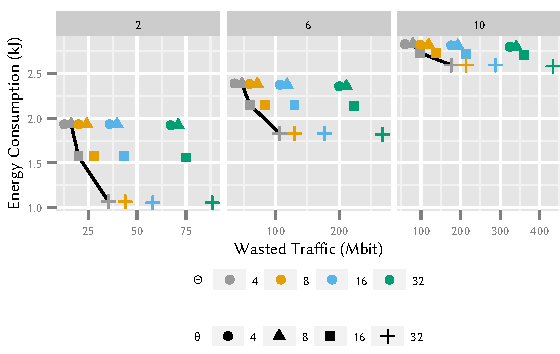
\includegraphics{application/lte_video/trade_offs/figures/energy2lostData}
  \caption{Evaluation of the streaming mechanism for varying video bitrates regarding energy consumption and wasted traffic}
  \label{fig:application:lte_video:numerical_evaluation:trade_offs:energy2lostData}
\end{figure}


First, we consider the trade-off between energy consumption and wasted traffic in \reffig{fig:application:lte_video:numerical_evaluation:trade_offs:energy2lostData}.
We find that, independent of video bitrate, the values found on the Pareto frontier can be obtained for the smallest considered buffer threshold.
Increasing the buffer size decreases the energy consumption at the cost of a higher wasted traffic.
Choosing a small lower buffer threshold \bufferlower decreases the minimum amount of wasted traffic if the user stops watching a video.
Selecting a higher buffer size \buffersize  increases the wasted traffic, as more video can be downloaded and thus wasted if a user stops watching the video.
Increasing the buffer size \buffersize decreases the energy consumption, because a longer buffer size allows for the video to be downloaded in fewer bursts and
each of them is followed by the \tidle timeout where the \gls{UE} is still in the most energy intensive \rrcconnected state.
For this trade-off, we recommend to always use the smallest possible stop threshold generating no stalling.
The choice of the buffer size depends on the preference between energy consumption and wasted bandwidth, with smaller threshold sizes requiring more energy and higher threshold sizes causing a higher wasted traffic.

\begin{figure}
  \centering
  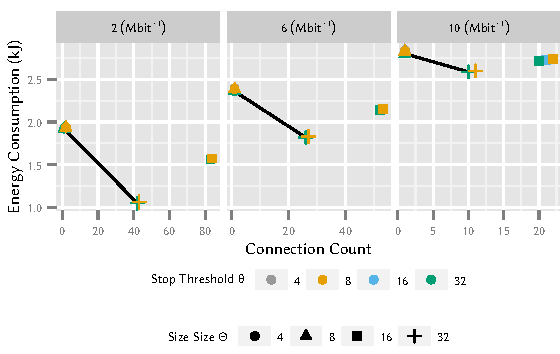
\includegraphics{application/lte_video/trade_offs/figures/energy2connections}
  \caption{Evaluation of the streaming mechanism for varying video bitrates regarding energy consumption and signalling}
  \label{fig:application:lte_video:numerical_evaluation:trade_offs:energy2connections}
\end{figure}

In \reffig{fig:application:lte_video:numerical_evaluation:trade_offs:energy2connections} we consider both the energy consumption as well as the connection count metric.
For all considered bitrate, the largest possible lower buffer threshold is pareto optimal.
A trade-off between energy consumption and connection count is possible by varying the buffer size.
A small buffer size yields a larger energy consumption and a smaller connection count while for a larger buffer size a smaller energy consumption and a higher connection count can be achieved.

\begin{figure}
  \centering
  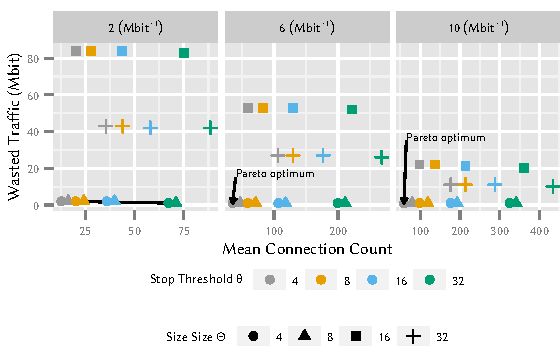
\includegraphics{application/lte_video/trade_offs/figures/connections2lostData}
  \caption{Evaluation of the streaming mechanism for varying video bitrates regarding signalling and wasted traffic}
  \label{fig:application:lte_video:numerical_evaluation:trade_offs:connections2lostData}
\end{figure}

Finally, in \reffig{fig:application:lte_video:numerical_evaluation:trade_offs:connections2lostData} we study the trade-off between the number of connections required per video transmission and the amount of lost data.
We observe, that for a bitrate of \SI{2}{\mega\bit\per\second} configurations exist where only one and two connections are required to transmit the complete video.
Here, the the amount of wasted traffic can be reduced by \SI{82}{\percent} by allowing just one more connection over the whole transmission interval.
For video bitrates of \SIlist{6;10}{\mega\bit\per\second} only one pareto optimal value exists where the video is transmitted using a single connection.

We find that each of the considered trade-offs provides pareto optimal results and summarize the relevant parameters qualitatively in \reftab{tab:application:lte_video:numerical_evaluation:trade_offs:summary}.
\begin{table}
  \centering
  \begin{tabular}{lcc}
    \toprule
    Trade-Off & Parameter & Optimal Value\\
    \midrule
    Wasted Traffic vs. Energy & Lower Buffer & Low\\
    Connection Count vs. Energy & Lower Buffer & High\\
    Wasted Traffic vs. Connection Count & Lower Buffer & Low\\
    \bottomrule
  \end{tabular}
  \caption{Qualitative results of trade-off analysis}
  \label{tab:application:lte_video:numerical_evaluation:trade_offs:summary}
\end{table}

From these results it becomes clear, that it is impossible to find pareto optimal results for all three trade-offs.
Thus, new decision making policies are required in order to find optimal results for all participating stakeholders.
One such policy will be discussed is \emph{Design for Tussle}~\cite{trilogy2008,Clark2005}.
Here, the attempts are made to resolve trade-offs and conflicts at run-time instead of design-time.
This way, the requirements of the stakeholders can be adapted to the current situation, e.g. an \gls{ISP} could require less stringent signalling bounds if the signalling load is currently low in the network.
Such functionalities could be implemented in the \glspl{UE} operating system, which even currently serves as a mediator between the different stakeholders.